% Created by tikzDevice version 0.6.2-92-0ad2792 on 2013-04-07 18:04:17
% !TEX encoding = UTF-8 Unicode
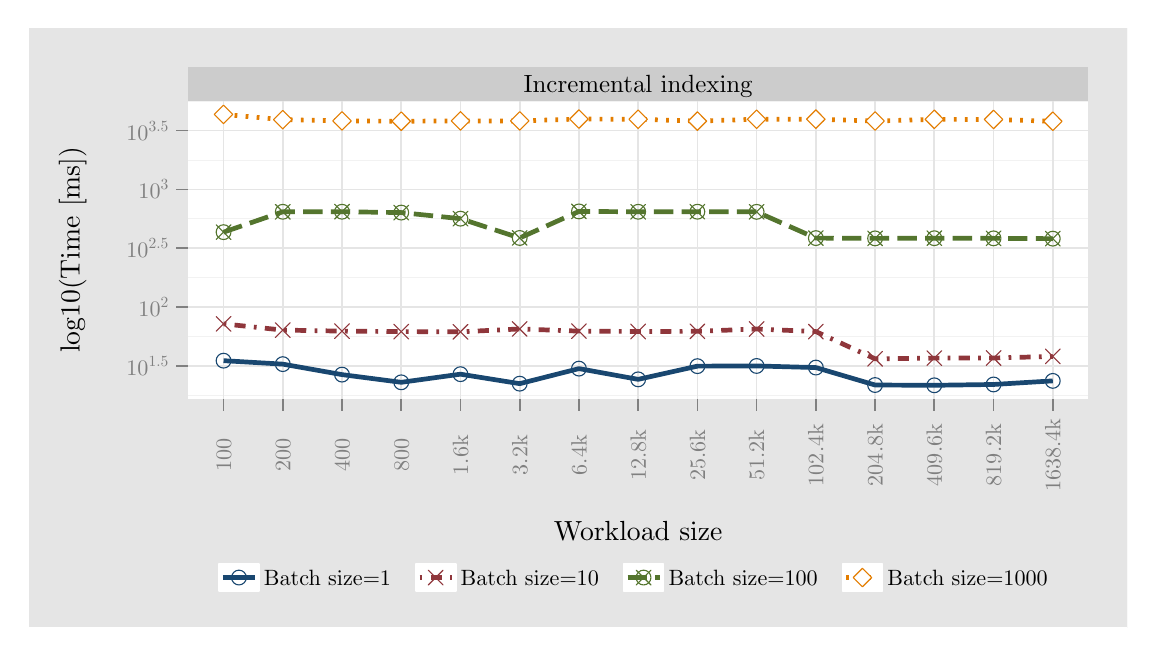
\begin{tikzpicture}[x=1pt,y=1pt]
\definecolor[named]{fillColor}{rgb}{1.00,1.00,1.00}
\path[use as bounding box,fill=fillColor,fill opacity=0.00] (0,0) rectangle (397.48,216.81);
\begin{scope}
\path[clip] (  0.00,  0.00) rectangle (397.48,216.81);
\definecolor[named]{drawColor}{rgb}{1.00,1.00,1.00}
\definecolor[named]{fillColor}{rgb}{0.90,0.90,0.90}

\path[draw=drawColor,line width= 0.6pt,line join=round,line cap=round,fill=fillColor] (  0.00,  0.00) rectangle (397.48,216.81);
\end{scope}
\begin{scope}
\path[clip] ( 57.94, 82.69) rectangle (383.26,190.36);
\definecolor[named]{fillColor}{rgb}{1.00,1.00,1.00}

\path[fill=fillColor] ( 57.94, 82.69) rectangle (383.26,190.36);
\definecolor[named]{drawColor}{rgb}{0.95,0.95,0.95}

\path[draw=drawColor,line width= 0.3pt,line join=round] ( 57.94, 84.04) --
	(383.26, 84.04);

\path[draw=drawColor,line width= 0.3pt,line join=round] ( 57.94,105.27) --
	(383.26,105.27);

\path[draw=drawColor,line width= 0.3pt,line join=round] ( 57.94,126.51) --
	(383.26,126.51);

\path[draw=drawColor,line width= 0.3pt,line join=round] ( 57.94,147.74) --
	(383.26,147.74);

\path[draw=drawColor,line width= 0.3pt,line join=round] ( 57.94,168.97) --
	(383.26,168.97);

\path[draw=drawColor,line width= 0.3pt,line join=round] ( 57.94,190.21) --
	(383.26,190.21);
\definecolor[named]{drawColor}{rgb}{0.90,0.90,0.90}

\path[draw=drawColor,line width= 0.6pt,line join=round] ( 57.94, 94.65) --
	(383.26, 94.65);

\path[draw=drawColor,line width= 0.6pt,line join=round] ( 57.94,115.89) --
	(383.26,115.89);

\path[draw=drawColor,line width= 0.6pt,line join=round] ( 57.94,137.12) --
	(383.26,137.12);

\path[draw=drawColor,line width= 0.6pt,line join=round] ( 57.94,158.36) --
	(383.26,158.36);

\path[draw=drawColor,line width= 0.6pt,line join=round] ( 57.94,179.59) --
	(383.26,179.59);

\path[draw=drawColor,line width= 0.6pt,line join=round] ( 70.78, 82.69) --
	( 70.78,190.36);

\path[draw=drawColor,line width= 0.6pt,line join=round] ( 92.18, 82.69) --
	( 92.18,190.36);

\path[draw=drawColor,line width= 0.6pt,line join=round] (113.58, 82.69) --
	(113.58,190.36);

\path[draw=drawColor,line width= 0.6pt,line join=round] (134.99, 82.69) --
	(134.99,190.36);

\path[draw=drawColor,line width= 0.6pt,line join=round] (156.39, 82.69) --
	(156.39,190.36);

\path[draw=drawColor,line width= 0.6pt,line join=round] (177.79, 82.69) --
	(177.79,190.36);

\path[draw=drawColor,line width= 0.6pt,line join=round] (199.20, 82.69) --
	(199.20,190.36);

\path[draw=drawColor,line width= 0.6pt,line join=round] (220.60, 82.69) --
	(220.60,190.36);

\path[draw=drawColor,line width= 0.6pt,line join=round] (242.00, 82.69) --
	(242.00,190.36);

\path[draw=drawColor,line width= 0.6pt,line join=round] (263.40, 82.69) --
	(263.40,190.36);

\path[draw=drawColor,line width= 0.6pt,line join=round] (284.81, 82.69) --
	(284.81,190.36);

\path[draw=drawColor,line width= 0.6pt,line join=round] (306.21, 82.69) --
	(306.21,190.36);

\path[draw=drawColor,line width= 0.6pt,line join=round] (327.61, 82.69) --
	(327.61,190.36);

\path[draw=drawColor,line width= 0.6pt,line join=round] (349.01, 82.69) --
	(349.01,190.36);

\path[draw=drawColor,line width= 0.6pt,line join=round] (370.42, 82.69) --
	(370.42,190.36);
\definecolor[named]{drawColor}{rgb}{0.10,0.28,0.44}

\path[draw=drawColor,line width= 1.7pt,line join=round] ( 70.78, 96.48) --
	( 92.18, 95.23) --
	(113.58, 91.44) --
	(134.99, 88.66) --
	(156.39, 91.60) --
	(177.79, 88.17) --
	(199.20, 93.61) --
	(220.60, 89.73) --
	(242.00, 94.50) --
	(263.40, 94.57) --
	(284.81, 93.99) --
	(306.21, 87.68) --
	(327.61, 87.58) --
	(349.01, 87.88) --
	(370.42, 89.18);
\definecolor[named]{drawColor}{rgb}{0.56,0.21,0.23}

\path[draw=drawColor,line width= 1.7pt,dash pattern=on 1pt off 3pt on 4pt off 3pt ,line join=round] ( 70.78,109.78) --
	( 92.18,107.53) --
	(113.58,107.16) --
	(134.99,106.99) --
	(156.39,106.91) --
	(177.79,107.94) --
	(199.20,107.16) --
	(220.60,107.03) --
	(242.00,107.08) --
	(263.40,107.93) --
	(284.81,106.99) --
	(306.21, 97.15) --
	(327.61, 97.40) --
	(349.01, 97.44) --
	(370.42, 98.02);
\definecolor[named]{drawColor}{rgb}{0.33,0.46,0.18}

\path[draw=drawColor,line width= 1.7pt,dash pattern=on 7pt off 3pt ,line join=round] ( 70.78,142.92) --
	( 92.18,150.28) --
	(113.58,150.30) --
	(134.99,149.99) --
	(156.39,147.79) --
	(177.79,140.82) --
	(199.20,150.41) --
	(220.60,150.28) --
	(242.00,150.30) --
	(263.40,150.26) --
	(284.81,140.77) --
	(306.21,140.67) --
	(327.61,140.73) --
	(349.01,140.68) --
	(370.42,140.57);
\definecolor[named]{drawColor}{rgb}{0.89,0.49,0.00}

\path[draw=drawColor,line width= 1.7pt,dash pattern=on 1pt off 3pt ,line join=round] ( 70.78,185.47) --
	( 92.18,183.57) --
	(113.58,183.10) --
	(134.99,183.00) --
	(156.39,183.12) --
	(177.79,183.12) --
	(199.20,183.79) --
	(220.60,183.71) --
	(242.00,183.04) --
	(263.40,183.73) --
	(284.81,183.75) --
	(306.21,183.07) --
	(327.61,183.68) --
	(349.01,183.64) --
	(370.42,182.99);
\definecolor[named]{drawColor}{rgb}{0.10,0.28,0.44}

\path[draw=drawColor,line width= 0.4pt,line join=round,line cap=round] ( 70.78, 96.48) circle (  2.67);
\definecolor[named]{drawColor}{rgb}{0.56,0.21,0.23}

\path[draw=drawColor,line width= 0.4pt,line join=round,line cap=round,fill=fillColor] ( 68.11,107.11) -- ( 73.45,112.45);

\path[draw=drawColor,line width= 0.4pt,line join=round,line cap=round,fill=fillColor] ( 68.11,112.45) -- ( 73.45,107.11);
\definecolor[named]{drawColor}{rgb}{0.33,0.46,0.18}

\path[draw=drawColor,line width= 0.4pt,line join=round,line cap=round] ( 70.78,142.92) circle (  2.67);

\path[draw=drawColor,line width= 0.4pt,line join=round,line cap=round] ( 68.11,140.25) -- ( 73.45,145.58);

\path[draw=drawColor,line width= 0.4pt,line join=round,line cap=round] ( 68.11,145.58) -- ( 73.45,140.25);
\definecolor[named]{drawColor}{rgb}{0.89,0.49,0.00}

\path[draw=drawColor,line width= 0.4pt,line join=round,line cap=round,fill=fillColor] ( 70.78,182.13) --
	( 74.12,185.47) --
	( 70.78,188.81) --
	( 67.44,185.47) --
	cycle;
\definecolor[named]{drawColor}{rgb}{0.10,0.28,0.44}

\path[draw=drawColor,line width= 0.4pt,line join=round,line cap=round] ( 92.18, 95.23) circle (  2.67);
\definecolor[named]{drawColor}{rgb}{0.56,0.21,0.23}

\path[draw=drawColor,line width= 0.4pt,line join=round,line cap=round,fill=fillColor] ( 89.51,104.86) -- ( 94.85,110.20);

\path[draw=drawColor,line width= 0.4pt,line join=round,line cap=round,fill=fillColor] ( 89.51,110.20) -- ( 94.85,104.86);
\definecolor[named]{drawColor}{rgb}{0.33,0.46,0.18}

\path[draw=drawColor,line width= 0.4pt,line join=round,line cap=round] ( 92.18,150.28) circle (  2.67);

\path[draw=drawColor,line width= 0.4pt,line join=round,line cap=round] ( 89.51,147.61) -- ( 94.85,152.95);

\path[draw=drawColor,line width= 0.4pt,line join=round,line cap=round] ( 89.51,152.95) -- ( 94.85,147.61);
\definecolor[named]{drawColor}{rgb}{0.89,0.49,0.00}

\path[draw=drawColor,line width= 0.4pt,line join=round,line cap=round,fill=fillColor] ( 92.18,180.23) --
	( 95.52,183.57) --
	( 92.18,186.91) --
	( 88.84,183.57) --
	cycle;
\definecolor[named]{drawColor}{rgb}{0.10,0.28,0.44}

\path[draw=drawColor,line width= 0.4pt,line join=round,line cap=round] (113.58, 91.44) circle (  2.67);
\definecolor[named]{drawColor}{rgb}{0.56,0.21,0.23}

\path[draw=drawColor,line width= 0.4pt,line join=round,line cap=round,fill=fillColor] (110.92,104.49) -- (116.25,109.83);

\path[draw=drawColor,line width= 0.4pt,line join=round,line cap=round,fill=fillColor] (110.92,109.83) -- (116.25,104.49);
\definecolor[named]{drawColor}{rgb}{0.33,0.46,0.18}

\path[draw=drawColor,line width= 0.4pt,line join=round,line cap=round] (113.58,150.30) circle (  2.67);

\path[draw=drawColor,line width= 0.4pt,line join=round,line cap=round] (110.92,147.64) -- (116.25,152.97);

\path[draw=drawColor,line width= 0.4pt,line join=round,line cap=round] (110.92,152.97) -- (116.25,147.64);
\definecolor[named]{drawColor}{rgb}{0.89,0.49,0.00}

\path[draw=drawColor,line width= 0.4pt,line join=round,line cap=round,fill=fillColor] (113.58,179.76) --
	(116.93,183.10) --
	(113.58,186.44) --
	(110.24,183.10) --
	cycle;
\definecolor[named]{drawColor}{rgb}{0.10,0.28,0.44}

\path[draw=drawColor,line width= 0.4pt,line join=round,line cap=round] (134.99, 88.66) circle (  2.67);
\definecolor[named]{drawColor}{rgb}{0.56,0.21,0.23}

\path[draw=drawColor,line width= 0.4pt,line join=round,line cap=round,fill=fillColor] (132.32,104.33) -- (137.65,109.66);

\path[draw=drawColor,line width= 0.4pt,line join=round,line cap=round,fill=fillColor] (132.32,109.66) -- (137.65,104.33);
\definecolor[named]{drawColor}{rgb}{0.33,0.46,0.18}

\path[draw=drawColor,line width= 0.4pt,line join=round,line cap=round] (134.99,149.99) circle (  2.67);

\path[draw=drawColor,line width= 0.4pt,line join=round,line cap=round] (132.32,147.32) -- (137.65,152.66);

\path[draw=drawColor,line width= 0.4pt,line join=round,line cap=round] (132.32,152.66) -- (137.65,147.32);
\definecolor[named]{drawColor}{rgb}{0.89,0.49,0.00}

\path[draw=drawColor,line width= 0.4pt,line join=round,line cap=round,fill=fillColor] (134.99,179.66) --
	(138.33,183.00) --
	(134.99,186.35) --
	(131.64,183.00) --
	cycle;
\definecolor[named]{drawColor}{rgb}{0.10,0.28,0.44}

\path[draw=drawColor,line width= 0.4pt,line join=round,line cap=round] (156.39, 91.60) circle (  2.67);
\definecolor[named]{drawColor}{rgb}{0.56,0.21,0.23}

\path[draw=drawColor,line width= 0.4pt,line join=round,line cap=round,fill=fillColor] (153.72,104.24) -- (159.06,109.58);

\path[draw=drawColor,line width= 0.4pt,line join=round,line cap=round,fill=fillColor] (153.72,109.58) -- (159.06,104.24);
\definecolor[named]{drawColor}{rgb}{0.33,0.46,0.18}

\path[draw=drawColor,line width= 0.4pt,line join=round,line cap=round] (156.39,147.79) circle (  2.67);

\path[draw=drawColor,line width= 0.4pt,line join=round,line cap=round] (153.72,145.13) -- (159.06,150.46);

\path[draw=drawColor,line width= 0.4pt,line join=round,line cap=round] (153.72,150.46) -- (159.06,145.13);
\definecolor[named]{drawColor}{rgb}{0.89,0.49,0.00}

\path[draw=drawColor,line width= 0.4pt,line join=round,line cap=round,fill=fillColor] (156.39,179.78) --
	(159.73,183.12) --
	(156.39,186.47) --
	(153.05,183.12) --
	cycle;
\definecolor[named]{drawColor}{rgb}{0.10,0.28,0.44}

\path[draw=drawColor,line width= 0.4pt,line join=round,line cap=round] (177.79, 88.17) circle (  2.67);
\definecolor[named]{drawColor}{rgb}{0.56,0.21,0.23}

\path[draw=drawColor,line width= 0.4pt,line join=round,line cap=round,fill=fillColor] (175.12,105.27) -- (180.46,110.60);

\path[draw=drawColor,line width= 0.4pt,line join=round,line cap=round,fill=fillColor] (175.12,110.60) -- (180.46,105.27);
\definecolor[named]{drawColor}{rgb}{0.33,0.46,0.18}

\path[draw=drawColor,line width= 0.4pt,line join=round,line cap=round] (177.79,140.82) circle (  2.67);

\path[draw=drawColor,line width= 0.4pt,line join=round,line cap=round] (175.12,138.15) -- (180.46,143.49);

\path[draw=drawColor,line width= 0.4pt,line join=round,line cap=round] (175.12,143.49) -- (180.46,138.15);
\definecolor[named]{drawColor}{rgb}{0.89,0.49,0.00}

\path[draw=drawColor,line width= 0.4pt,line join=round,line cap=round,fill=fillColor] (177.79,179.78) --
	(181.14,183.12) --
	(177.79,186.46) --
	(174.45,183.12) --
	cycle;
\definecolor[named]{drawColor}{rgb}{0.10,0.28,0.44}

\path[draw=drawColor,line width= 0.4pt,line join=round,line cap=round] (199.20, 93.61) circle (  2.67);
\definecolor[named]{drawColor}{rgb}{0.56,0.21,0.23}

\path[draw=drawColor,line width= 0.4pt,line join=round,line cap=round,fill=fillColor] (196.53,104.49) -- (201.86,109.83);

\path[draw=drawColor,line width= 0.4pt,line join=round,line cap=round,fill=fillColor] (196.53,109.83) -- (201.86,104.49);
\definecolor[named]{drawColor}{rgb}{0.33,0.46,0.18}

\path[draw=drawColor,line width= 0.4pt,line join=round,line cap=round] (199.20,150.41) circle (  2.67);

\path[draw=drawColor,line width= 0.4pt,line join=round,line cap=round] (196.53,147.75) -- (201.86,153.08);

\path[draw=drawColor,line width= 0.4pt,line join=round,line cap=round] (196.53,153.08) -- (201.86,147.75);
\definecolor[named]{drawColor}{rgb}{0.89,0.49,0.00}

\path[draw=drawColor,line width= 0.4pt,line join=round,line cap=round,fill=fillColor] (199.20,180.44) --
	(202.54,183.79) --
	(199.20,187.13) --
	(195.85,183.79) --
	cycle;
\definecolor[named]{drawColor}{rgb}{0.10,0.28,0.44}

\path[draw=drawColor,line width= 0.4pt,line join=round,line cap=round] (220.60, 89.73) circle (  2.67);
\definecolor[named]{drawColor}{rgb}{0.56,0.21,0.23}

\path[draw=drawColor,line width= 0.4pt,line join=round,line cap=round,fill=fillColor] (217.93,104.36) -- (223.27,109.70);

\path[draw=drawColor,line width= 0.4pt,line join=round,line cap=round,fill=fillColor] (217.93,109.70) -- (223.27,104.36);
\definecolor[named]{drawColor}{rgb}{0.33,0.46,0.18}

\path[draw=drawColor,line width= 0.4pt,line join=round,line cap=round] (220.60,150.28) circle (  2.67);

\path[draw=drawColor,line width= 0.4pt,line join=round,line cap=round] (217.93,147.62) -- (223.27,152.95);

\path[draw=drawColor,line width= 0.4pt,line join=round,line cap=round] (217.93,152.95) -- (223.27,147.62);
\definecolor[named]{drawColor}{rgb}{0.89,0.49,0.00}

\path[draw=drawColor,line width= 0.4pt,line join=round,line cap=round,fill=fillColor] (220.60,180.36) --
	(223.94,183.71) --
	(220.60,187.05) --
	(217.25,183.71) --
	cycle;
\definecolor[named]{drawColor}{rgb}{0.10,0.28,0.44}

\path[draw=drawColor,line width= 0.4pt,line join=round,line cap=round] (242.00, 94.50) circle (  2.67);
\definecolor[named]{drawColor}{rgb}{0.56,0.21,0.23}

\path[draw=drawColor,line width= 0.4pt,line join=round,line cap=round,fill=fillColor] (239.33,104.41) -- (244.67,109.75);

\path[draw=drawColor,line width= 0.4pt,line join=round,line cap=round,fill=fillColor] (239.33,109.75) -- (244.67,104.41);
\definecolor[named]{drawColor}{rgb}{0.33,0.46,0.18}

\path[draw=drawColor,line width= 0.4pt,line join=round,line cap=round] (242.00,150.30) circle (  2.67);

\path[draw=drawColor,line width= 0.4pt,line join=round,line cap=round] (239.33,147.64) -- (244.67,152.97);

\path[draw=drawColor,line width= 0.4pt,line join=round,line cap=round] (239.33,152.97) -- (244.67,147.64);
\definecolor[named]{drawColor}{rgb}{0.89,0.49,0.00}

\path[draw=drawColor,line width= 0.4pt,line join=round,line cap=round,fill=fillColor] (242.00,179.70) --
	(245.34,183.04) --
	(242.00,186.39) --
	(238.66,183.04) --
	cycle;
\definecolor[named]{drawColor}{rgb}{0.10,0.28,0.44}

\path[draw=drawColor,line width= 0.4pt,line join=round,line cap=round] (263.40, 94.57) circle (  2.67);
\definecolor[named]{drawColor}{rgb}{0.56,0.21,0.23}

\path[draw=drawColor,line width= 0.4pt,line join=round,line cap=round,fill=fillColor] (260.74,105.26) -- (266.07,110.60);

\path[draw=drawColor,line width= 0.4pt,line join=round,line cap=round,fill=fillColor] (260.74,110.60) -- (266.07,105.26);
\definecolor[named]{drawColor}{rgb}{0.33,0.46,0.18}

\path[draw=drawColor,line width= 0.4pt,line join=round,line cap=round] (263.40,150.26) circle (  2.67);

\path[draw=drawColor,line width= 0.4pt,line join=round,line cap=round] (260.74,147.60) -- (266.07,152.93);

\path[draw=drawColor,line width= 0.4pt,line join=round,line cap=round] (260.74,152.93) -- (266.07,147.60);
\definecolor[named]{drawColor}{rgb}{0.89,0.49,0.00}

\path[draw=drawColor,line width= 0.4pt,line join=round,line cap=round,fill=fillColor] (263.40,180.39) --
	(266.75,183.73) --
	(263.40,187.08) --
	(260.06,183.73) --
	cycle;
\definecolor[named]{drawColor}{rgb}{0.10,0.28,0.44}

\path[draw=drawColor,line width= 0.4pt,line join=round,line cap=round] (284.81, 93.99) circle (  2.67);
\definecolor[named]{drawColor}{rgb}{0.56,0.21,0.23}

\path[draw=drawColor,line width= 0.4pt,line join=round,line cap=round,fill=fillColor] (282.14,104.32) -- (287.47,109.65);

\path[draw=drawColor,line width= 0.4pt,line join=round,line cap=round,fill=fillColor] (282.14,109.65) -- (287.47,104.32);
\definecolor[named]{drawColor}{rgb}{0.33,0.46,0.18}

\path[draw=drawColor,line width= 0.4pt,line join=round,line cap=round] (284.81,140.77) circle (  2.67);

\path[draw=drawColor,line width= 0.4pt,line join=round,line cap=round] (282.14,138.11) -- (287.47,143.44);

\path[draw=drawColor,line width= 0.4pt,line join=round,line cap=round] (282.14,143.44) -- (287.47,138.11);
\definecolor[named]{drawColor}{rgb}{0.89,0.49,0.00}

\path[draw=drawColor,line width= 0.4pt,line join=round,line cap=round,fill=fillColor] (284.81,180.41) --
	(288.15,183.75) --
	(284.81,187.10) --
	(281.46,183.75) --
	cycle;
\definecolor[named]{drawColor}{rgb}{0.10,0.28,0.44}

\path[draw=drawColor,line width= 0.4pt,line join=round,line cap=round] (306.21, 87.68) circle (  2.67);
\definecolor[named]{drawColor}{rgb}{0.56,0.21,0.23}

\path[draw=drawColor,line width= 0.4pt,line join=round,line cap=round,fill=fillColor] (303.54, 94.48) -- (308.88, 99.81);

\path[draw=drawColor,line width= 0.4pt,line join=round,line cap=round,fill=fillColor] (303.54, 99.81) -- (308.88, 94.48);
\definecolor[named]{drawColor}{rgb}{0.33,0.46,0.18}

\path[draw=drawColor,line width= 0.4pt,line join=round,line cap=round] (306.21,140.67) circle (  2.67);

\path[draw=drawColor,line width= 0.4pt,line join=round,line cap=round] (303.54,138.01) -- (308.88,143.34);

\path[draw=drawColor,line width= 0.4pt,line join=round,line cap=round] (303.54,143.34) -- (308.88,138.01);
\definecolor[named]{drawColor}{rgb}{0.89,0.49,0.00}

\path[draw=drawColor,line width= 0.4pt,line join=round,line cap=round,fill=fillColor] (306.21,179.73) --
	(309.55,183.07) --
	(306.21,186.42) --
	(302.87,183.07) --
	cycle;
\definecolor[named]{drawColor}{rgb}{0.10,0.28,0.44}

\path[draw=drawColor,line width= 0.4pt,line join=round,line cap=round] (327.61, 87.58) circle (  2.67);
\definecolor[named]{drawColor}{rgb}{0.56,0.21,0.23}

\path[draw=drawColor,line width= 0.4pt,line join=round,line cap=round,fill=fillColor] (324.94, 94.73) -- (330.28,100.07);

\path[draw=drawColor,line width= 0.4pt,line join=round,line cap=round,fill=fillColor] (324.94,100.07) -- (330.28, 94.73);
\definecolor[named]{drawColor}{rgb}{0.33,0.46,0.18}

\path[draw=drawColor,line width= 0.4pt,line join=round,line cap=round] (327.61,140.73) circle (  2.67);

\path[draw=drawColor,line width= 0.4pt,line join=round,line cap=round] (324.94,138.07) -- (330.28,143.40);

\path[draw=drawColor,line width= 0.4pt,line join=round,line cap=round] (324.94,143.40) -- (330.28,138.07);
\definecolor[named]{drawColor}{rgb}{0.89,0.49,0.00}

\path[draw=drawColor,line width= 0.4pt,line join=round,line cap=round,fill=fillColor] (327.61,180.34) --
	(330.95,183.68) --
	(327.61,187.03) --
	(324.27,183.68) --
	cycle;
\definecolor[named]{drawColor}{rgb}{0.10,0.28,0.44}

\path[draw=drawColor,line width= 0.4pt,line join=round,line cap=round] (349.01, 87.88) circle (  2.67);
\definecolor[named]{drawColor}{rgb}{0.56,0.21,0.23}

\path[draw=drawColor,line width= 0.4pt,line join=round,line cap=round,fill=fillColor] (346.35, 94.77) -- (351.68,100.11);

\path[draw=drawColor,line width= 0.4pt,line join=round,line cap=round,fill=fillColor] (346.35,100.11) -- (351.68, 94.77);
\definecolor[named]{drawColor}{rgb}{0.33,0.46,0.18}

\path[draw=drawColor,line width= 0.4pt,line join=round,line cap=round] (349.01,140.68) circle (  2.67);

\path[draw=drawColor,line width= 0.4pt,line join=round,line cap=round] (346.35,138.02) -- (351.68,143.35);

\path[draw=drawColor,line width= 0.4pt,line join=round,line cap=round] (346.35,143.35) -- (351.68,138.02);
\definecolor[named]{drawColor}{rgb}{0.89,0.49,0.00}

\path[draw=drawColor,line width= 0.4pt,line join=round,line cap=round,fill=fillColor] (349.01,180.29) --
	(352.36,183.64) --
	(349.01,186.98) --
	(345.67,183.64) --
	cycle;
\definecolor[named]{drawColor}{rgb}{0.10,0.28,0.44}

\path[draw=drawColor,line width= 0.4pt,line join=round,line cap=round] (370.42, 89.18) circle (  2.67);
\definecolor[named]{drawColor}{rgb}{0.56,0.21,0.23}

\path[draw=drawColor,line width= 0.4pt,line join=round,line cap=round,fill=fillColor] (367.75, 95.35) -- (373.08,100.69);

\path[draw=drawColor,line width= 0.4pt,line join=round,line cap=round,fill=fillColor] (367.75,100.69) -- (373.08, 95.35);
\definecolor[named]{drawColor}{rgb}{0.33,0.46,0.18}

\path[draw=drawColor,line width= 0.4pt,line join=round,line cap=round] (370.42,140.57) circle (  2.67);

\path[draw=drawColor,line width= 0.4pt,line join=round,line cap=round] (367.75,137.90) -- (373.08,143.23);

\path[draw=drawColor,line width= 0.4pt,line join=round,line cap=round] (367.75,143.23) -- (373.08,137.90);
\definecolor[named]{drawColor}{rgb}{0.89,0.49,0.00}

\path[draw=drawColor,line width= 0.4pt,line join=round,line cap=round,fill=fillColor] (370.42,179.65) --
	(373.76,182.99) --
	(370.42,186.34) --
	(367.07,182.99) --
	cycle;
\end{scope}
\begin{scope}
\path[clip] (  0.00,  0.00) rectangle (397.48,216.81);
\definecolor[named]{fillColor}{rgb}{0.80,0.80,0.80}

\path[fill=fillColor] ( 57.94,190.36) rectangle (383.26,202.58);
\definecolor[named]{drawColor}{rgb}{0.00,0.00,0.00}

\node[text=drawColor,anchor=base,inner sep=0pt, outer sep=0pt, scale=  0.90] at (220.60,193.37) {Incremental indexing};
\end{scope}
\begin{scope}
\path[clip] (  0.00,  0.00) rectangle (397.48,216.81);
\definecolor[named]{drawColor}{rgb}{0.50,0.50,0.50}

\node[text=drawColor,anchor=base west,inner sep=0pt, outer sep=0pt, scale=  0.80] at ( 35.67, 91.22) {10};

\node[text=drawColor,anchor=base west,inner sep=0pt, outer sep=0pt, scale=  0.56] at ( 43.67, 94.49) {1};

\node[text=drawColor,anchor=base west,inner sep=0pt, outer sep=0pt, scale=  0.56] at ( 46.47, 94.49) {.};

\node[text=drawColor,anchor=base west,inner sep=0pt, outer sep=0pt, scale=  0.56] at ( 48.02, 94.49) {5};

\node[text=drawColor,anchor=base west,inner sep=0pt, outer sep=0pt, scale=  0.80] at ( 40.03,112.46) {10};

\node[text=drawColor,anchor=base west,inner sep=0pt, outer sep=0pt, scale=  0.56] at ( 48.02,115.73) {2};

\node[text=drawColor,anchor=base west,inner sep=0pt, outer sep=0pt, scale=  0.80] at ( 35.67,133.69) {10};

\node[text=drawColor,anchor=base west,inner sep=0pt, outer sep=0pt, scale=  0.56] at ( 43.67,136.96) {2};

\node[text=drawColor,anchor=base west,inner sep=0pt, outer sep=0pt, scale=  0.56] at ( 46.47,136.96) {.};

\node[text=drawColor,anchor=base west,inner sep=0pt, outer sep=0pt, scale=  0.56] at ( 48.02,136.96) {5};

\node[text=drawColor,anchor=base west,inner sep=0pt, outer sep=0pt, scale=  0.80] at ( 40.03,154.93) {10};

\node[text=drawColor,anchor=base west,inner sep=0pt, outer sep=0pt, scale=  0.56] at ( 48.02,158.20) {3};

\node[text=drawColor,anchor=base west,inner sep=0pt, outer sep=0pt, scale=  0.80] at ( 35.67,176.16) {10};

\node[text=drawColor,anchor=base west,inner sep=0pt, outer sep=0pt, scale=  0.56] at ( 43.67,179.43) {3};

\node[text=drawColor,anchor=base west,inner sep=0pt, outer sep=0pt, scale=  0.56] at ( 46.47,179.43) {.};

\node[text=drawColor,anchor=base west,inner sep=0pt, outer sep=0pt, scale=  0.56] at ( 48.02,179.43) {5};
\end{scope}
\begin{scope}
\path[clip] (  0.00,  0.00) rectangle (397.48,216.81);
\definecolor[named]{drawColor}{rgb}{0.50,0.50,0.50}

\path[draw=drawColor,line width= 0.6pt,line join=round] ( 53.67, 94.65) --
	( 57.94, 94.65);

\path[draw=drawColor,line width= 0.6pt,line join=round] ( 53.67,115.89) --
	( 57.94,115.89);

\path[draw=drawColor,line width= 0.6pt,line join=round] ( 53.67,137.12) --
	( 57.94,137.12);

\path[draw=drawColor,line width= 0.6pt,line join=round] ( 53.67,158.36) --
	( 57.94,158.36);

\path[draw=drawColor,line width= 0.6pt,line join=round] ( 53.67,179.59) --
	( 57.94,179.59);
\end{scope}
\begin{scope}
\path[clip] (  0.00,  0.00) rectangle (397.48,216.81);
\definecolor[named]{drawColor}{rgb}{0.50,0.50,0.50}

\path[draw=drawColor,line width= 0.6pt,line join=round] ( 70.78, 78.42) --
	( 70.78, 82.69);

\path[draw=drawColor,line width= 0.6pt,line join=round] ( 92.18, 78.42) --
	( 92.18, 82.69);

\path[draw=drawColor,line width= 0.6pt,line join=round] (113.58, 78.42) --
	(113.58, 82.69);

\path[draw=drawColor,line width= 0.6pt,line join=round] (134.99, 78.42) --
	(134.99, 82.69);

\path[draw=drawColor,line width= 0.6pt,line join=round] (156.39, 78.42) --
	(156.39, 82.69);

\path[draw=drawColor,line width= 0.6pt,line join=round] (177.79, 78.42) --
	(177.79, 82.69);

\path[draw=drawColor,line width= 0.6pt,line join=round] (199.20, 78.42) --
	(199.20, 82.69);

\path[draw=drawColor,line width= 0.6pt,line join=round] (220.60, 78.42) --
	(220.60, 82.69);

\path[draw=drawColor,line width= 0.6pt,line join=round] (242.00, 78.42) --
	(242.00, 82.69);

\path[draw=drawColor,line width= 0.6pt,line join=round] (263.40, 78.42) --
	(263.40, 82.69);

\path[draw=drawColor,line width= 0.6pt,line join=round] (284.81, 78.42) --
	(284.81, 82.69);

\path[draw=drawColor,line width= 0.6pt,line join=round] (306.21, 78.42) --
	(306.21, 82.69);

\path[draw=drawColor,line width= 0.6pt,line join=round] (327.61, 78.42) --
	(327.61, 82.69);

\path[draw=drawColor,line width= 0.6pt,line join=round] (349.01, 78.42) --
	(349.01, 82.69);

\path[draw=drawColor,line width= 0.6pt,line join=round] (370.42, 78.42) --
	(370.42, 82.69);
\end{scope}
\begin{scope}
\path[clip] (  0.00,  0.00) rectangle (397.48,216.81);
\definecolor[named]{drawColor}{rgb}{0.50,0.50,0.50}

\node[text=drawColor,rotate= 90.00,anchor=base,inner sep=0pt, outer sep=0pt, scale=  0.80] at ( 73.53, 62.36) {100};

\node[text=drawColor,rotate= 90.00,anchor=base,inner sep=0pt, outer sep=0pt, scale=  0.80] at ( 94.94, 62.36) {200};

\node[text=drawColor,rotate= 90.00,anchor=base,inner sep=0pt, outer sep=0pt, scale=  0.80] at (116.34, 62.36) {400};

\node[text=drawColor,rotate= 90.00,anchor=base,inner sep=0pt, outer sep=0pt, scale=  0.80] at (137.74, 62.36) {800};

\node[text=drawColor,rotate= 90.00,anchor=base,inner sep=0pt, outer sep=0pt, scale=  0.80] at (159.14, 62.36) {1.6k};

\node[text=drawColor,rotate= 90.00,anchor=base,inner sep=0pt, outer sep=0pt, scale=  0.80] at (180.55, 62.36) {3.2k};

\node[text=drawColor,rotate= 90.00,anchor=base,inner sep=0pt, outer sep=0pt, scale=  0.80] at (201.95, 62.36) {6.4k};

\node[text=drawColor,rotate= 90.00,anchor=base,inner sep=0pt, outer sep=0pt, scale=  0.80] at (223.35, 62.36) {12.8k};

\node[text=drawColor,rotate= 90.00,anchor=base,inner sep=0pt, outer sep=0pt, scale=  0.80] at (244.76, 62.36) {25.6k};

\node[text=drawColor,rotate= 90.00,anchor=base,inner sep=0pt, outer sep=0pt, scale=  0.80] at (266.16, 62.36) {51.2k};

\node[text=drawColor,rotate= 90.00,anchor=base,inner sep=0pt, outer sep=0pt, scale=  0.80] at (287.56, 62.36) {102.4k};

\node[text=drawColor,rotate= 90.00,anchor=base,inner sep=0pt, outer sep=0pt, scale=  0.80] at (308.96, 62.36) {204.8k};

\node[text=drawColor,rotate= 90.00,anchor=base,inner sep=0pt, outer sep=0pt, scale=  0.80] at (330.37, 62.36) {409.6k};

\node[text=drawColor,rotate= 90.00,anchor=base,inner sep=0pt, outer sep=0pt, scale=  0.80] at (351.77, 62.36) {819.2k};

\node[text=drawColor,rotate= 90.00,anchor=base,inner sep=0pt, outer sep=0pt, scale=  0.80] at (373.17, 62.36) {1638.4k};
\end{scope}
\begin{scope}
\path[clip] (  0.00,  0.00) rectangle (397.48,216.81);
\definecolor[named]{drawColor}{rgb}{0.00,0.00,0.00}

\node[text=drawColor,anchor=base,inner sep=0pt, outer sep=0pt, scale=  1.00] at (220.60, 31.41) {Workload size};
\end{scope}
\begin{scope}
\path[clip] (  0.00,  0.00) rectangle (397.48,216.81);
\definecolor[named]{drawColor}{rgb}{0.00,0.00,0.00}

\node[text=drawColor,rotate= 90.00,anchor=base,inner sep=0pt, outer sep=0pt, scale=  1.00] at ( 18.80,136.53) {log10(Time [ms])};
\end{scope}
\begin{scope}
\path[clip] (  0.00,  0.00) rectangle (397.48,216.81);
\definecolor[named]{fillColor}{rgb}{0.90,0.90,0.90}

\path[fill=fillColor] ( 61.23,  8.87) rectangle (379.97, 27.36);
\end{scope}
\begin{scope}
\path[clip] (  0.00,  0.00) rectangle (397.48,216.81);
\definecolor[named]{drawColor}{rgb}{1.00,1.00,1.00}
\definecolor[named]{fillColor}{rgb}{1.00,1.00,1.00}

\path[draw=drawColor,line width= 0.6pt,line join=round,line cap=round,fill=fillColor] ( 69.11, 13.14) rectangle ( 83.56, 23.09);
\end{scope}
\begin{scope}
\path[clip] (  0.00,  0.00) rectangle (397.48,216.81);
\definecolor[named]{drawColor}{rgb}{0.10,0.28,0.44}

\path[draw=drawColor,line width= 1.7pt,line join=round] ( 70.56, 18.11) -- ( 82.12, 18.11);
\end{scope}
\begin{scope}
\path[clip] (  0.00,  0.00) rectangle (397.48,216.81);
\definecolor[named]{drawColor}{rgb}{0.10,0.28,0.44}

\path[draw=drawColor,line width= 0.4pt,line join=round,line cap=round] ( 76.34, 18.11) circle (  2.67);
\end{scope}
\begin{scope}
\path[clip] (  0.00,  0.00) rectangle (397.48,216.81);
\definecolor[named]{drawColor}{rgb}{1.00,1.00,1.00}
\definecolor[named]{fillColor}{rgb}{1.00,1.00,1.00}

\path[draw=drawColor,line width= 0.6pt,line join=round,line cap=round,fill=fillColor] (140.21, 13.14) rectangle (154.66, 23.09);
\end{scope}
\begin{scope}
\path[clip] (  0.00,  0.00) rectangle (397.48,216.81);
\definecolor[named]{drawColor}{rgb}{0.56,0.21,0.23}

\path[draw=drawColor,line width= 1.7pt,dash pattern=on 1pt off 3pt on 4pt off 3pt ,line join=round] (141.66, 18.11) -- (153.22, 18.11);
\end{scope}
\begin{scope}
\path[clip] (  0.00,  0.00) rectangle (397.48,216.81);
\definecolor[named]{drawColor}{rgb}{0.56,0.21,0.23}
\definecolor[named]{fillColor}{rgb}{1.00,1.00,1.00}

\path[draw=drawColor,line width= 0.4pt,line join=round,line cap=round,fill=fillColor] (144.77, 15.45) -- (150.11, 20.78);

\path[draw=drawColor,line width= 0.4pt,line join=round,line cap=round,fill=fillColor] (144.77, 20.78) -- (150.11, 15.45);
\end{scope}
\begin{scope}
\path[clip] (  0.00,  0.00) rectangle (397.48,216.81);
\definecolor[named]{drawColor}{rgb}{1.00,1.00,1.00}
\definecolor[named]{fillColor}{rgb}{1.00,1.00,1.00}

\path[draw=drawColor,line width= 0.6pt,line join=round,line cap=round,fill=fillColor] (215.31, 13.14) rectangle (229.76, 23.09);
\end{scope}
\begin{scope}
\path[clip] (  0.00,  0.00) rectangle (397.48,216.81);
\definecolor[named]{drawColor}{rgb}{0.33,0.46,0.18}

\path[draw=drawColor,line width= 1.7pt,dash pattern=on 7pt off 3pt ,line join=round] (216.76, 18.11) -- (228.32, 18.11);
\end{scope}
\begin{scope}
\path[clip] (  0.00,  0.00) rectangle (397.48,216.81);
\definecolor[named]{drawColor}{rgb}{0.33,0.46,0.18}

\path[draw=drawColor,line width= 0.4pt,line join=round,line cap=round] (222.54, 18.11) circle (  2.67);

\path[draw=drawColor,line width= 0.4pt,line join=round,line cap=round] (219.87, 15.45) -- (225.20, 20.78);

\path[draw=drawColor,line width= 0.4pt,line join=round,line cap=round] (219.87, 20.78) -- (225.20, 15.45);
\end{scope}
\begin{scope}
\path[clip] (  0.00,  0.00) rectangle (397.48,216.81);
\definecolor[named]{drawColor}{rgb}{1.00,1.00,1.00}
\definecolor[named]{fillColor}{rgb}{1.00,1.00,1.00}

\path[draw=drawColor,line width= 0.6pt,line join=round,line cap=round,fill=fillColor] (294.41, 13.14) rectangle (308.86, 23.09);
\end{scope}
\begin{scope}
\path[clip] (  0.00,  0.00) rectangle (397.48,216.81);
\definecolor[named]{drawColor}{rgb}{0.89,0.49,0.00}

\path[draw=drawColor,line width= 1.7pt,dash pattern=on 1pt off 3pt ,line join=round] (295.85, 18.11) -- (307.42, 18.11);
\end{scope}
\begin{scope}
\path[clip] (  0.00,  0.00) rectangle (397.48,216.81);
\definecolor[named]{drawColor}{rgb}{0.89,0.49,0.00}
\definecolor[named]{fillColor}{rgb}{1.00,1.00,1.00}

\path[draw=drawColor,line width= 0.4pt,line join=round,line cap=round,fill=fillColor] (301.64, 14.77) --
	(304.98, 18.11) --
	(301.64, 21.46) --
	(298.29, 18.11) --
	cycle;
\end{scope}
\begin{scope}
\path[clip] (  0.00,  0.00) rectangle (397.48,216.81);
\definecolor[named]{drawColor}{rgb}{0.00,0.00,0.00}

\node[text=drawColor,anchor=base west,inner sep=0pt, outer sep=0pt, scale=  0.80] at ( 85.37, 15.36) {Batch size=1 $\;\;$};
\end{scope}
\begin{scope}
\path[clip] (  0.00,  0.00) rectangle (397.48,216.81);
\definecolor[named]{drawColor}{rgb}{0.00,0.00,0.00}

\node[text=drawColor,anchor=base west,inner sep=0pt, outer sep=0pt, scale=  0.80] at (156.47, 15.36) {Batch size=10 $\;\;$};
\end{scope}
\begin{scope}
\path[clip] (  0.00,  0.00) rectangle (397.48,216.81);
\definecolor[named]{drawColor}{rgb}{0.00,0.00,0.00}

\node[text=drawColor,anchor=base west,inner sep=0pt, outer sep=0pt, scale=  0.80] at (231.57, 15.36) {Batch size=100 $\;\;$};
\end{scope}
\begin{scope}
\path[clip] (  0.00,  0.00) rectangle (397.48,216.81);
\definecolor[named]{drawColor}{rgb}{0.00,0.00,0.00}

\node[text=drawColor,anchor=base west,inner sep=0pt, outer sep=0pt, scale=  0.80] at (310.67, 15.36) {Batch size=1000 $\;\;$};
\end{scope}
\end{tikzpicture}
